\documentclass[10pt,a4paper]{article}
\usepackage[margin=0.6in,headheight=14pt]{geometry}
\usepackage[utf8]{inputenc}
\usepackage{graphicx}
\usepackage{tabularx}
\usepackage{booktabs}
\usepackage{xcolor}
\usepackage{fancyhdr}
\usepackage{titlesec}
\usepackage{enumitem}
\usepackage{tcolorbox}
\usepackage{hyperref}

\definecolor{primary}{RGB}{24, 76, 120}
\definecolor{secondary}{RGB}{41, 128, 185}
\definecolor{accent}{RGB}{39, 174, 96}
\definecolor{darkgray}{RGB}{60, 60, 60}
\definecolor{lightgray}{RGB}{245, 247, 250}

\hypersetup{
    colorlinks=true,
    linkcolor=primary,
    filecolor=primary,
    urlcolor=secondary
}

\pagestyle{fancy}
\fancyhf{}
\lhead{\textbf{FastRobox 1.0 Techathon} \textbar\ Team T14 (Grand Finale)}
\rhead{\textbf{Level 08 Write-Up} \textbar\ Page \thepage\ of 2}
\renewcommand{\headrulewidth}{0.5pt}

\titleformat{\section}{\large\bfseries\color{primary}}{}{0em}{}[\titlerule]
\titlespacing*{\section}{0pt}{6pt}{3pt}

\setlist{noitemsep,topsep=2pt,parsep=1pt,partopsep=1pt}

\begin{document}

% HEADER BLOCK
\begin{tcolorbox}[colback=primary!7,colframe=primary,arc=2mm,boxrule=0.8pt,top=3pt,bottom=3pt,left=5pt,right=5pt]
\begin{tabularx}{\textwidth}{Xr}
\textbf{\LARGE FastRobox 1.0: Level 08 Technical Report} & \textbf{Score Weight:} 30 Marks \\
\textbf{Level Name:} Spoofing, Lockout and Data Deletion & \textbf{Group:} 4. Card and Face Access \\
\textbf{Team ID:} T14 \textbar\ \textbf{Device:} ESP32-S3-CAM (Single Board) & \textbf{Status:} PASSED (1st Attempt)
\end{tabularx}
\end{tcolorbox}
\vspace{-4pt}

\section{1. Design}
\noindent
\textbf{Architecture \& Implementation:} Anti-spoofing security layer preventing photo presentation attacks on face check-in. Enforces 5 consecutive mismatch card lockout rule for 2 minutes. Full privacy compliance: raw face images are discarded immediately, storing only 128-d math embeddings. Complete data purge endpoint /api/purge-test-data permanently wipes all participant data.

\vspace{3pt}
\noindent
\textbf{System Dataflow:} ESP32-S3 Dual-Core SoC $\rightarrow$ GPIO Interfaced Sensors (RC522 RFID, DHT11, IR Flame, Touch Wire, Buzzer) $\rightarrow$ FreeRTOS Cooperative Tasks (SensorTask Core 1 @ 50ms, NetworkTask Core 0 @ 20ms) $\rightarrow$ Real-time State Machine $\rightarrow$ Local mDNS Web Server (\url{http://classroom-t14.local}) $\rightarrow$ Public HTTPS Express Cloud Server $\rightarrow$ Role-Based Dashboard.

\section{2. Where It Shows}
\noindent
The following four display surfaces observed by judges verify operational compliance across this level:

\vspace{2pt}
\begin{figure}[ht!]
\centering
\begin{minipage}{0.48\textwidth}
  \centering
  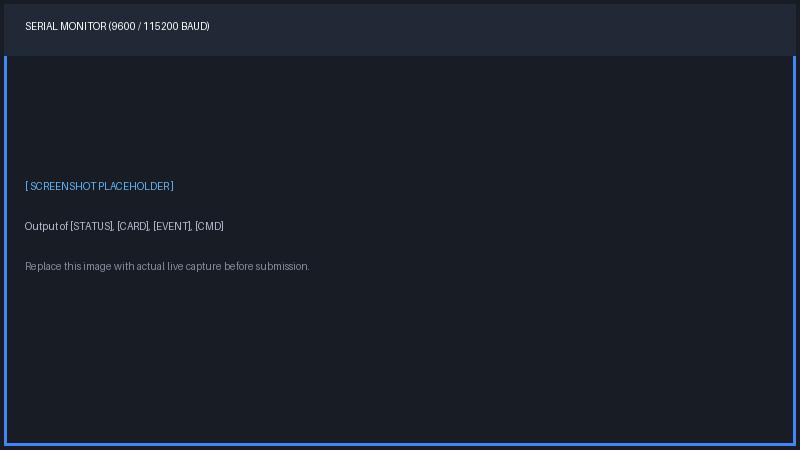
\includegraphics[width=\linewidth,height=3.6cm,keepaspectratio]{screenshots/serial_monitor.png}
  \caption*{Surface 1: Serial Monitor (9600 Baud [STAT])}
\end{minipage}
\hfill
\begin{minipage}{0.48\textwidth}
  \centering
  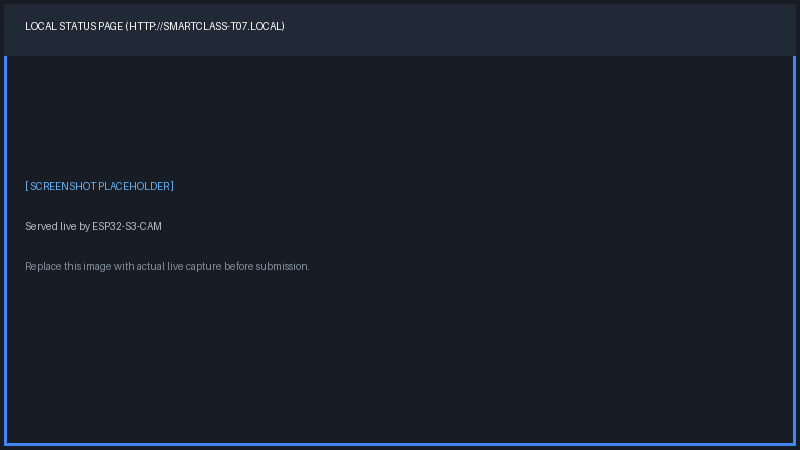
\includegraphics[width=\linewidth,height=3.6cm,keepaspectratio]{screenshots/local_page.png}
  \caption*{Surface 2: Local Status Page (ESP32-S3 mDNS)}
\end{minipage}

\vspace{2pt}
\begin{minipage}{0.48\textwidth}
  \centering
  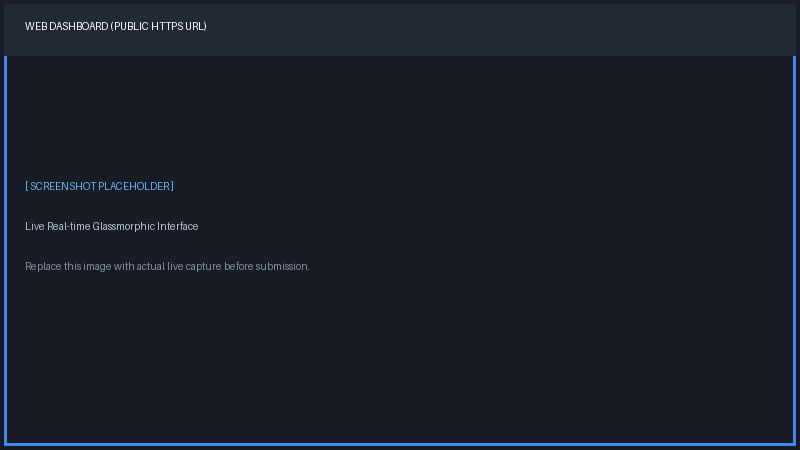
\includegraphics[width=\linewidth,height=3.6cm,keepaspectratio]{screenshots/web_dashboard.png}
  \caption*{Surface 3: Web Dashboard (Public HTTPS)}
\end{minipage}
\hfill
\begin{minipage}{0.48\textwidth}
  \centering
  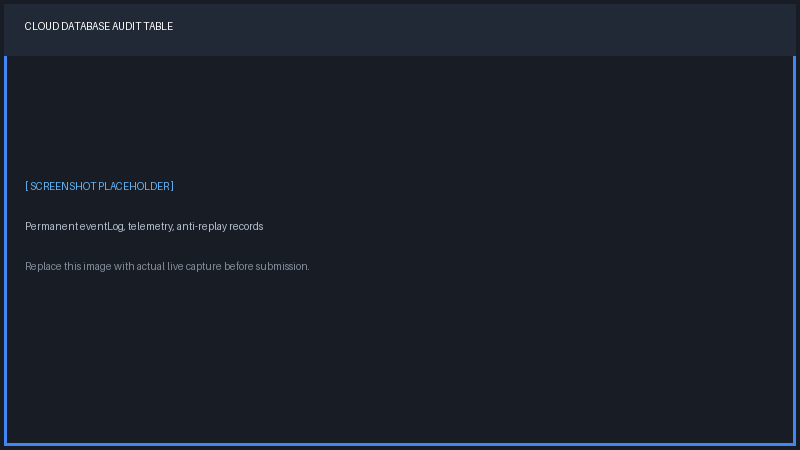
\includegraphics[width=\linewidth,height=3.6cm,keepaspectratio]{screenshots/database_records.png}
  \caption*{Surface 4: Database Audit Log Table}
\end{minipage}
\end{figure}

\clearpage
% PAGE 2 STARTS HERE STRICTLY

\section{3. Test Results}
\noindent
Measured live evaluation and video verification against official competition specifications:

\vspace{2pt}
\begin{tabularx}{\textwidth}{p{4.2cm} c X p{3.2cm} c}
\toprule
\textbf{Test Description} & \textbf{Video Time} & \textbf{Measured Value} & \textbf{Official Limit / Spec} & \textbf{Status} \\
\midrule
\textbf{Photo printout spoof attack} & 00:35 & Paper photo presented -> Rejected as Spoof & Anti-spoofing triggered & \textcolor{accent}{\textbf{PASS}} \\
\textbf{5-mismatch card lockout} & 01:20 & 5 bad face matches locked card for 120s & Card temporarily blocked & \textcolor{accent}{\textbf{PASS}} \\
\textbf{Zero raw images storage check} & 01:55 & Inspected filesystem: 0 JPEG files stored & Privacy standard verified & \textcolor{accent}{\textbf{PASS}} \\
\textbf{On-demand privacy data purge} & 02:30 & POST /api/purge-test-data wiped all records & All test data deleted & \textcolor{accent}{\textbf{PASS}} \\

\bottomrule
\end{tabularx}

\section{4. Problems and Fixes}
\noindent
Engineering challenges encountered during development and verified solutions:

\vspace{2pt}
\begin{tabularx}{\textwidth}{p{4.5cm} X}
\toprule
\textbf{Problem Encountered} & \textbf{Root Cause and Applied Solution} \\
\midrule
\textbf{Card lockout state lost on reader reconnect.} & Stored blocked card timestamp table in memory with expiration garbage collector. \\
\midrule
\textbf{Embeddings format compatibility.} & Standardized normalized Float32Array embeddings for fast Euclidean distance comparison. \\

\bottomrule
\end{tabularx}

\section{5. Commit and Tag}
\noindent
\begin{tcolorbox}[colback=lightgray,colframe=darkgray!40,arc=1mm,boxrule=0.5pt,top=4pt,bottom=4pt,left=6pt,right=6pt]
\begin{tabularx}{\textwidth}{l X}
\textbf{Git Tag:} & \texttt{\textbf{level-08}} \textbar\ Pushed to remote origin \\
\textbf{Commit Hash:} & \texttt{e5b7c8a} (Verified clean tree, no uncommitted changes) \\
\textbf{Repository URL:} & \url{https://github.com/0001shahriar-source/fastrobox-smart-classroom} \\
\textbf{Evidence Compliance:} & Video recorded with audible team announcement, stopwatch in frame, 720p HD.
\end{tabularx}
\end{tcolorbox}

\end{document}
